% Does Random Mean Secure?
% Randomness, Predictability and Information Leakage
%
% A 20-minute talk built as one argument: what randomness means, how we
% test for it, what the tests miss, and what predictability costs once the
% random bits become an encryption key.
%
% Theme: Singapore (structure + top navigation), with hand-made
% Boadilla-like compact list markers and a purple palette.
% Compile with pdflatex (twice) or latexmk.

\documentclass[11pt,aspectratio=169]{beamer}
\usetheme{Singapore}
\usefonttheme{professionalfonts}

\usepackage[T1]{fontenc}
\usepackage{cmbright}
\usepackage{amsmath,amssymb}
\usepackage{booktabs}
\usepackage{tikz}
\usepackage{pgfplots}
\pgfplotsset{compat=1.18}
\usetikzlibrary{arrows.meta,positioning,calc}

% Notation.
\newcommand{\Prob}[1]{\mathbb{P}\!\left(#1\right)}
\newcommand{\Ex}[1]{\mathbb{E}\!\left[#1\right]}
\newcommand{\Var}[1]{\operatorname{Var}\!\left(#1\right)}
\newcommand{\Ent}[1]{H\!\left(#1\right)}          % entropy
\newcommand{\CEnt}[2]{H\!\left(#1 \mid #2\right)} % conditional entropy
\newcommand{\MI}[2]{I\!\left(#1 ; #2\right)}      % mutual information
\newcommand{\msg}{M}
\newcommand{\key}{K}
\newcommand{\ctxt}{C}
\newcommand{\xor}{\oplus}
\newcommand{\bits}{\{0,1\}}
\newcommand{\Bern}{\mathrm{Bern}}
\newcommand{\Bin}{\mathrm{Bin}}

% ---------------------------------------------------------------------------
% Palette
% ---------------------------------------------------------------------------
\definecolor{deep}{HTML}{3F2860}
\definecolor{primary}{HTML}{6C4AB6}
\definecolor{secondary}{HTML}{8063C5}
\definecolor{lavender}{HTML}{DDD3F2}
\definecolor{verylight}{HTML}{F5F1FB}
\definecolor{paper}{HTML}{FCFBFE}
\definecolor{ink}{HTML}{211B2B}
\definecolor{muted}{HTML}{70697A}

\setbeamercolor{background canvas}{bg=paper}
\setbeamercolor{normal text}{fg=ink,bg=paper}
\setbeamercolor{structure}{fg=deep}
\setbeamercolor{title}{fg=deep}
\setbeamercolor{subtitle}{fg=muted}
\setbeamercolor{author}{fg=ink}
\setbeamercolor{date}{fg=muted}
\setbeamercolor{frametitle}{fg=deep}
\setbeamercolor{framesubtitle}{fg=muted}
\setbeamercolor{alerted text}{fg=primary}
\setbeamercolor{section in head/foot}{fg=deep,bg=verylight}
\setbeamercolor{mini frame}{fg=primary}
\setbeamercolor{block title}{fg=deep,bg=lavender}
\setbeamercolor{block body}{fg=ink,bg=verylight}
\setbeamercolor{footline}{fg=muted}

% ---------------------------------------------------------------------------
% Navigation: Singapore's mini frames at the top, only the five sections.
% ---------------------------------------------------------------------------
\setbeamertemplate{navigation symbols}{}
\setbeamertemplate{footline}{%
  \hfill{\scriptsize\color{muted}\insertframenumber}\hspace{1em}\vskip1ex}

% Frame heading: small technical label, narrative title, optional subtitle.
\setbeamerfont{title}{size=\LARGE,series=\bfseries}
\setbeamerfont{subtitle}{size=\large}
\setbeamerfont{frametitle}{size=\Large,series=\bfseries}
\setbeamerfont{framesubtitle}{size=\normalsize,series=\mdseries}
\makeatletter
\setbeamersize{text margin left=0.6cm,text margin right=0.6cm}
\setbeamertemplate{frametitle}{%
  \vskip0.2ex
  {\footnotesize\bfseries\color{muted}%
    \MakeUppercase{\insertsectionhead}%
    \ifx\insertsubsectionhead\@empty\else
      \ \textperiodcentered\ \MakeUppercase{\insertsubsectionhead}\fi\par}
  \vskip0.2ex
  {\usebeamerfont{frametitle}\usebeamercolor[fg]{frametitle}\insertframetitle\par}
  \ifx\insertframesubtitle\@empty\else
    {\vskip0.2ex\usebeamerfont{framesubtitle}\usebeamercolor[fg]{framesubtitle}\insertframesubtitle\par}\fi
  \vskip0.1ex
}
% Tighter display-math spacing than the article defaults.
\g@addto@macro\normalsize{%
  \setlength{\abovedisplayskip}{4pt}\setlength{\belowdisplayskip}{4pt}%
  \setlength{\abovedisplayshortskip}{2pt}\setlength{\belowdisplayshortskip}{2pt}}
\g@addto@macro\small{%
  \setlength{\abovedisplayskip}{3pt}\setlength{\belowdisplayskip}{3pt}%
  \setlength{\abovedisplayshortskip}{2pt}\setlength{\belowdisplayshortskip}{2pt}}
\makeatother

% ---------------------------------------------------------------------------
% Lists: compact Boadilla-like markers, drawn by hand so Singapore stays.
% ---------------------------------------------------------------------------
\setbeamertemplate{itemize item}{%
  \tikz[baseline=-0.55ex]\fill[primary] (0,0) circle (1.4pt);}
\setbeamertemplate{itemize subitem}{%
  \tikz[baseline=-0.55ex]\draw[secondary,line width=0.6pt] (0,0) circle (1.1pt);}
\setbeamertemplate{enumerate item}{%
  \tikz[baseline=-0.7ex]{\fill[primary] (0,0) circle (1.05em/2);
    \node[white,font=\scriptsize\bfseries] at (0,0) {\insertenumlabel};}}
\setbeamertemplate{enumerate subitem}{%
  \textcolor{secondary}{\scriptsize\insertsubenumlabel.}}
\setlength{\leftmargini}{1.4em}
\setlength{\leftmarginii}{1.3em}
\setbeamertemplate{itemize/enumerate body begin}{\setlength{\itemsep}{0.35ex}}
\setbeamertemplate{itemize/enumerate subbody begin}{\setlength{\itemsep}{0.2ex}}
\setbeamertemplate{blocks}[rounded][shadow=false]

% ---------------------------------------------------------------------------
% Small helpers
% ---------------------------------------------------------------------------
% Bit strings: 1 in purple, 0 in grey, | as a run separator.
\makeatletter
\newcommand{\bitstring}[1]{{\ttfamily\@tfor\bt:=#1\do{%
  \if\bt1\textcolor{primary}{1}\else\if\bt|\textcolor{muted}{\,|\,}\else\textcolor{muted}{0}\fi\fi}}}
\makeatother
% A tinted callout box.
\newcommand{\callout}[1]{%
  \begin{center}\begin{tikzpicture}
    \node[fill=verylight,draw=lavender,rounded corners=4pt,inner sep=8pt,
          text width=0.86\textwidth,align=center]{#1};
  \end{tikzpicture}\end{center}}
\newcommand{\keyeq}[1]{\begin{center}\large\color{deep}$\displaystyle #1$\end{center}}

\title{Does Random Mean Secure?}
\subtitle{Randomness, Predictability and Information Leakage}
\author{tdvnm}
\institute{Probability and Statistics project}
\date{\today}

\begin{document}

% ===========================================================================
% 1. Title
% ===========================================================================
\begin{frame}[plain]
  \titlepage
\end{frame}

% ===========================================================================
\section{Randomness}
% ===========================================================================

% 2. Opening: get the audience to produce a "random" string, then ask
%    whether their choices were really random. Creates the question the
%    next slide answers.
\begin{frame}{Can we actually make something random?}
  \framesubtitle{Try it: write down 10--15 zeros and ones, as randomly as you can.}
  \vspace{0.5ex}
  \begin{center}
    {\Huge\bitstring{101001011010010}}
  \end{center}
  \vspace{1ex}
  \begin{itemize}
    \item Did you deliberately balance the zeros and ones?
    \item Did you avoid \bitstring{0000} or \bitstring{1111}?
    \item Did you alternate more than a coin would?
  \end{itemize}
  \vspace{1ex}
  \callout{Our sense of what \emph{looks} random is not a probability model.\\
    So what should a genuinely random source actually do?}
\end{frame}

% 3. The ideal model: fair and independent bits, and the two ways to fail.
\begin{frame}{So what should a random sequence actually do?}
  \framesubtitle{Model the source as bits $B_1,\ldots,B_n\in\bits$.}
  \begin{columns}[T]
    \begin{column}{0.48\textwidth}
      \textbf{\color{deep}Fairness}\\
      No preference for 0 or 1.
      \[\Prob{B_i=1}=\Prob{B_i=0}=\tfrac12\]
      \textbf{\color{deep}Independence}\\
      Knowing earlier bits does not help predict the next one.
      \[\Prob{B_{i+1}=1\mid B_1,\ldots,B_i}=\Prob{B_{i+1}=1}\]
    \end{column}
    \begin{column}{0.48\textwidth}
      \begin{block}{Two ways this can fail}
        \textbf{Bias.} The probabilities of 0 and 1 are wrong.

        \medskip
        \textbf{Dependence.} The counts may look fine, but the bits
        influence one another.
      \end{block}
      \medskip
      Under this model every $n$-bit string has probability $2^{-n}$.
      A test compares the data against exactly that.
    \end{column}
  \end{columns}
\end{frame}

% ===========================================================================
\section{Testing}
\subsection{Frequency Test}
% ===========================================================================

% 4. Frequency test: same counts, different structure. Bin(n,1/2) appears
%    because we count successes in independent Bernoulli trials.
\begin{frame}{Half zeros and half ones is not enough}
  \framesubtitle{Both strings have eight zeros and eight ones.}
  \begin{center}
    {\LARGE\bitstring{0000000011111111}}\\[0.6ex]
    {\LARGE\bitstring{0101010101010101}}
  \end{center}
  The frequency is right in both. The pattern clearly is not.
  \smallskip
  \begin{columns}[T]
    \begin{column}{0.5\textwidth}
      Count the ones:
      \[X=\sum_{i=1}^{n}B_i\]
      Under independent fair bits,
      \[X\sim\Bin(n,\tfrac12).\]
    \end{column}
    \begin{column}{0.46\textwidth}
      \begin{block}{The frequency test asks}
        Is the observed number of ones unusual under the fair-bit model?
      \end{block}
      \medskip
      It cannot see order at all. A correct frequency does not imply
      independence.
    \end{column}
  \end{columns}
\end{frame}

\subsection{Runs Test}

% 5. Runs test: a statistic that does see order.
\begin{frame}{Two tests ask two different questions}
  \framesubtitle{Frequency measures balance. Runs measure pattern.}
  A \emph{run} is a maximal block of equal bits:
  \begin{center}
    {\LARGE\bitstring{0011100}}\quad$\longrightarrow$\quad
    {\LARGE\bitstring{00|111|00}}\qquad three runs
  \end{center}
  \smallskip
  \begin{columns}[T]
    \begin{column}{0.5\textwidth}
      \[R=1+\#\{\text{switches }B_i\ne B_{i+1}\}\]
      Each of the $n-1$ neighbouring pairs switches independently with
      probability $\tfrac12$, so
      \[R-1\sim\Bin(n-1,\tfrac12).\]
    \end{column}
    \begin{column}{0.46\textwidth}
      \begin{block}{Frequency test}
        Is the balance of zeros and ones unusual?
      \end{block}
      \begin{block}{Runs test}
        Is the amount of switching or repeating unusual?
      \end{block}
    \end{column}
  \end{columns}
  \smallskip
  Two sequences can share a frequency and still differ completely in
  dependence.
\end{frame}

% 6. Dependence, modelled: a two-state Markov chain with switching
%    probability s. Only the Markov property is used. This is NOT the key
%    model of the later experiment; that one changes bias, not dependence.
\begin{frame}{What if randomness has memory?}
  \framesubtitle{A source whose next bit depends only on its current bit.}
  \begin{columns}[T]
    \begin{column}{0.42\textwidth}
      \begin{center}
        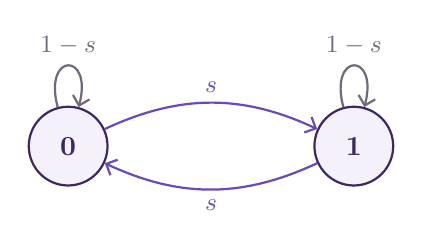
\begin{tikzpicture}[>={Straight Barb},node distance=2.6cm,
            state/.style={circle,draw=deep,fill=verylight,thick,
                          minimum size=1cm,font=\bfseries\color{deep}}]
          \node[state] (z) {0};
          \node[state,right=of z] (o) {1};
          \draw[->,primary,thick] (z) to[bend left=25] node[above,font=\small] {$s$} (o);
          \draw[->,primary,thick] (o) to[bend left=25] node[below,font=\small] {$s$} (z);
          \draw[->,muted,thick] (z) to[loop above,looseness=7] node[above,font=\small] {$1-s$} (z);
          \draw[->,muted,thick] (o) to[loop above,looseness=7] node[above,font=\small] {$1-s$} (o);
        \end{tikzpicture}
      \end{center}
      \[P=\begin{pmatrix}1-s&s\\ s&1-s\end{pmatrix}\]
      {\small $s$ = probability of switching}
    \end{column}
    \begin{column}{0.54\textwidth}
      \textbf{\color{deep}$s=0.5$}\quad the current bit says nothing
      about the next: independent fair bits.

      \smallskip
      \textbf{\color{deep}$s=0.8$}\quad the next bit is probably the
      opposite of this one.

      \smallskip
      Started symmetrically, both keep roughly half zeros and half ones.
      Only the switching changes: $\Ex{R}=1+(n-1)s$.
      \begin{block}{}
        50/50 does not imply independence. The frequency test passes;
        the runs test is the one that notices.
      \end{block}
    \end{column}
  \end{columns}
\end{frame}

% ===========================================================================
\section{Predictability}
\subsection{Pseudorandom Generators}
% ===========================================================================

% 7. The gap: what a test result means, and why "passes tests" is a weaker
%    statement than "cannot be predicted".
\begin{frame}{Looking random is not the same as being unpredictable}
  A $p$-value asks: \emph{if the ideal model were true, how unusual would a
  statistic this extreme be?} Small: evidence against the model.
  Large: this test found nothing. That is not proof of security.
  \medskip
  \begin{columns}[T]
    \begin{column}{0.48\textwidth}
      \textbf{\color{deep}Statistical question}\\
      Does the observed output behave like the probability model?
    \end{column}
    \begin{column}{0.48\textwidth}
      \textbf{\color{deep}Security question}\\
      Can someone predict future output, or recover the generator's state?
    \end{column}
  \end{columns}
  \medskip
  A pseudorandom generator is a deterministic rule on a hidden state,
  \[S_{n+1}=f(S_n),\qquad B_n=g(S_n).\]
  Its output can look convincing on a finite sample; recover the state and
  every future bit is fixed. Cryptographic generators (Linux's
  \texttt{getrandom()}) are deterministic after seeding too; their design
  goal is that prediction is infeasible. Passing tests does not show that.
\end{frame}

% ===========================================================================
\section{Secrecy}
\subsection{XOR}
% ===========================================================================

% 8. Transition: predictability was a property of a sequence; now the
%    sequence is a key. Two-bit XOR so the whole model is exactly computable.
\begin{frame}{What happens when randomness becomes a key?}
  \framesubtitle{So far, predictability was a property of a sequence. Now use the bits as a key.}
  \begin{columns}[T]
    \begin{column}{0.44\textwidth}
      \keyeq{\ctxt=\msg\xor\key}
      \begin{center}
        {\Large\ttfamily
        \begin{tabular}{@{}lc@{}}
          \color{muted}Message    & 0\,1 \\
          \color{muted}Key        & 1\,0 \\
          \midrule
          \color{deep}Ciphertext & \color{deep}1\,1
        \end{tabular}}
      \end{center}
      XOR is its own inverse, so the receiver applies the same key again:
      $11\xor10=01$.
    \end{column}
    \begin{column}{0.52\textwidth}
      \begin{block}{Why two bits}
        Four messages, four keys, four ciphertexts. The whole probability
        model is a $4\times4$ table, so everything that follows is an
        exact calculation, not an estimate.
      \end{block}
      \smallskip
      The attacker sees $\ctxt$ and knows the rule and the distributions of
      $\msg$ and $\key$, but not the key that was used.
    \end{column}
  \end{columns}
\end{frame}

\subsection{Perfect Secrecy}

% 9. Perfect secrecy stated in words first, then shown for the uniform key
%    with one line of conditional probability.
\begin{frame}{When does the ciphertext tell us nothing?}
  \framesubtitle{Seeing the ciphertext should not change what the attacker believes.}
  \keyeq{\Prob{\msg=m\mid\ctxt=c}=\Prob{\msg=m}}
  \begin{columns}[T]
    \begin{column}{0.5\textwidth}
      Take a uniform, independent two-bit key:
      \[\Prob{\key=00}=\Prob{01}=\Prob{10}=\Prob{11}=\tfrac14.\]
      For any message $m$ and ciphertext $c$ there is exactly one key
      that connects them, $k=m\xor c$. So
      \[\Prob{\ctxt=c\mid\msg=m}=\Prob{\key=m\xor c}=\tfrac14\]
      for every $m$.
    \end{column}
    \begin{column}{0.46\textwidth}
      \begin{block}{Then Bayes' rule finishes it}
        The likelihood $\Prob{\ctxt=c\mid\msg=m}$ is the same for every
        $m$, so it cancels: the posterior equals the prior.
      \end{block}
      \smallskip
      Every message explains every ciphertext equally well, so the
      ciphertext says nothing about which one was sent.
    \end{column}
  \end{columns}
\end{frame}

\subsection{Entropy \textperiodcentered\ Information Leakage}

% 10. Entropy as uncertainty, three worked bits, then mutual information as
%     "reduction in uncertainty about M after seeing C".
\begin{frame}{How do we measure what gets revealed?}
  \framesubtitle{Entropy is uncertainty, in bits. Leakage is how much of it disappears.}
  \begin{columns}[T]
    \begin{column}{0.4\textwidth}
      \begin{center}
        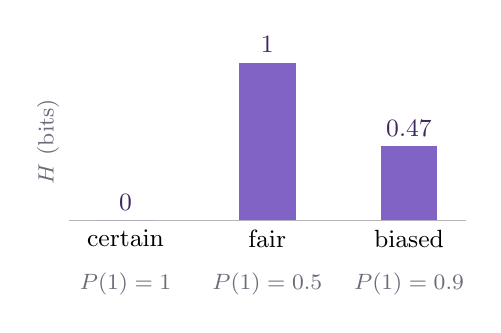
\begin{tikzpicture}[x=0.9cm,y=2cm]
          \draw[muted!50] (-0.3,0) -- (5.3,0);
          \foreach \x/\h/\lab/\p in {0.5/0/$0$/certain, 2.5/1/$1$/fair, 4.5/0.47/$0.47$/biased}{
            \fill[secondary] (\x-0.4,0) rectangle (\x+0.4,\h);
            \node[above,font=\small\color{deep}] at (\x,\h) {\lab};
            \node[below,font=\small,align=center] at (\x,0) {\p};
          }
          \node[below=0.55cm,font=\footnotesize\color{muted}] at (0.5,0) {$P(1)=1$};
          \node[below=0.55cm,font=\footnotesize\color{muted}] at (2.5,0) {$P(1)=0.5$};
          \node[below=0.55cm,font=\footnotesize\color{muted}] at (4.5,0) {$P(1)=0.9$};
          \node[left,font=\footnotesize\color{muted},rotate=90,anchor=south] at (-0.3,0.5) {$H$ (bits)};
        \end{tikzpicture}
      \end{center}
    \end{column}
    \begin{column}{0.56\textwidth}
      $\Ent{\msg}$: uncertainty about the message before seeing anything.

      $\CEnt{\msg}{\ctxt}$: uncertainty that remains after seeing the
      ciphertext.
      \keyeq{\MI{\msg}{\ctxt}=\Ent{\msg}-\CEnt{\msg}{\ctxt}}
      \begin{block}{Mutual information}
        How much the ciphertext reduces the attacker's uncertainty about
        the message. $\MI{\msg}{\ctxt}=0$: nothing leaked, perfect secrecy.
      \end{block}
    \end{column}
  \end{columns}
\end{frame}

% ===========================================================================
\section{Experiment}
\subsection{Experiment}
% ===========================================================================

% 11. The experiment: everything fixed except the key distribution.
%     Bias, not dependence; this is deliberately not the Markov source.
\begin{frame}{What if I change only the randomness?}
  \framesubtitle{Same cipher, same messages. Only the key distribution moves.}
  \vspace{-1ex}
  \begin{columns}[T]
    \begin{column}{0.48\textwidth}
      \begin{block}{Kept fixed}
        \begin{itemize}
          \item $\Prob{\msg=00,01,10,11}=(0.4,\,0.3,\,0.2,\,0.1)$
          \item $\ctxt=\msg\xor\key$, key independent of $\msg$
        \end{itemize}
      \end{block}
    \end{column}
    \begin{column}{0.48\textwidth}
      \begin{block}{Changed}
        \begin{itemize}
          \item $K_1,K_2$ independent $\Bern(q)$
          \item $q=0.50,\,0.55,\,\ldots,\,0.95$
        \end{itemize}
      \end{block}
    \end{column}
  \end{columns}
  \smallskip
  At $q=0.5$ this is the uniform key of the perfect-secrecy slide. As $q$
  grows the key bits still ignore each other; each just leans towards 1.
  \callout{A different failure from the Markov source: that example had
    \emph{dependence} with fair counts. Here the key bits stay independent
    and we turn up the \emph{bias}.}
\end{frame}

% 12. Make the degradation visible: the four key probabilities at the two
%     endpoints, then one concrete posterior so leakage is a belief change.
\begin{frame}{As the key becomes predictable, secrecy begins to disappear}
  \framesubtitle{At $q=0.95$ one key shows up nine times out of ten.}
  \begin{columns}[T]
    \begin{column}{0.5\textwidth}
      \begin{center}
        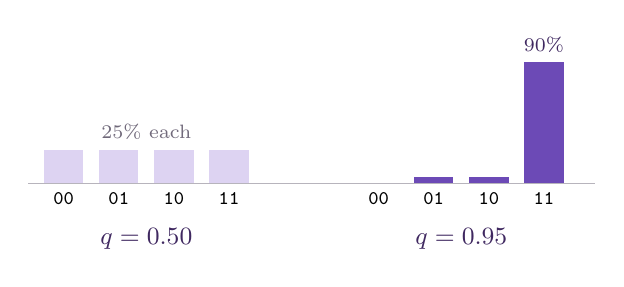
\begin{tikzpicture}[x=1cm,y=1.7cm]
          % q = 0.5
          \foreach \i/\k in {0/00,1/01,2/10,3/11}{
            \fill[lavender] (\i*0.7,0) rectangle (\i*0.7+0.5,0.25);
            \node[below,font=\scriptsize\ttfamily] at (\i*0.7+0.25,0) {\k};
          }
          \node[above,font=\scriptsize\color{muted}] at (1.3,0.25) {25\% each};
          \node[below=0.45cm,font=\small\color{deep}] at (1.3,0) {$q=0.50$};
          % q = 0.95
          \foreach \i/\k/\h in {0/00/0.0025,1/01/0.0475,2/10/0.0475,3/11/0.9025}{
            \fill[primary] (4+\i*0.7,0) rectangle (4+\i*0.7+0.5,\h);
            \node[below,font=\scriptsize\ttfamily] at (4+\i*0.7+0.25,0) {\k};
          }
          \node[above,font=\scriptsize\color{deep}] at (6.35,0.9025) {90\%};
          \node[below=0.45cm,font=\small\color{deep}] at (5.3,0) {$q=0.95$};
          \draw[muted!50] (-0.2,0) -- (7,0);
        \end{tikzpicture}
      \end{center}
      \smallskip
      Key entropy $\Ent{\key}=2h(q)$, with $h$ the entropy of one
      $\Bern(q)$ bit, falls from $2$ bits to $0.57$ bits.
    \end{column}
    \begin{column}{0.46\textwidth}
      \textbf{\color{deep}One ciphertext, $q=0.95$, $\ctxt=11$}
      \begin{center}
        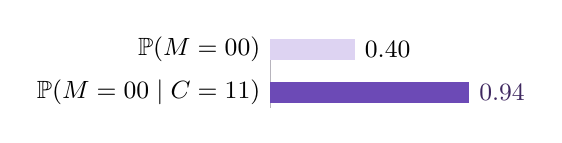
\begin{tikzpicture}[x=2.7cm,y=0.55cm]
          \draw[muted!50] (0,-0.1) -- (0,1.5);
          \fill[lavender] (0,1) rectangle (0.40,1.5);
          \node[right,font=\small] at (0.40,1.25) {$0.40$};
          \node[left,font=\small,align=right] at (0,1.25) {$\Prob{\msg=00}$};
          \fill[primary] (0,0) rectangle (0.938,0.5);
          \node[right,font=\small\color{deep}] at (0.938,0.25) {$0.94$};
          \node[left,font=\small,align=right] at (0,0.25) {$\Prob{\msg=00\mid\ctxt=11}$};
        \end{tikzpicture}
      \end{center}
      Before: ``00'' with probability $0.40$. After seeing $11$: $0.94$,
      because the key was almost surely $11$.
      \medskip

      \textbf{\color{deep}The ciphertext changed the attacker's belief.
      That change is the leakage we measure.}
    \end{column}
  \end{columns}
\end{frame}

\subsection{Results}

% 13. The main result: exact leakage and key entropy as q moves. Includes
%     the one-line derivation used to compute it.
\begin{frame}{The weaker the key, the more the ciphertext reveals}
  \framesubtitle{Exact calculation. Cipher and messages unchanged; only the key distribution moved.}
  \begin{columns}[T]
    \begin{column}{0.56\textwidth}
      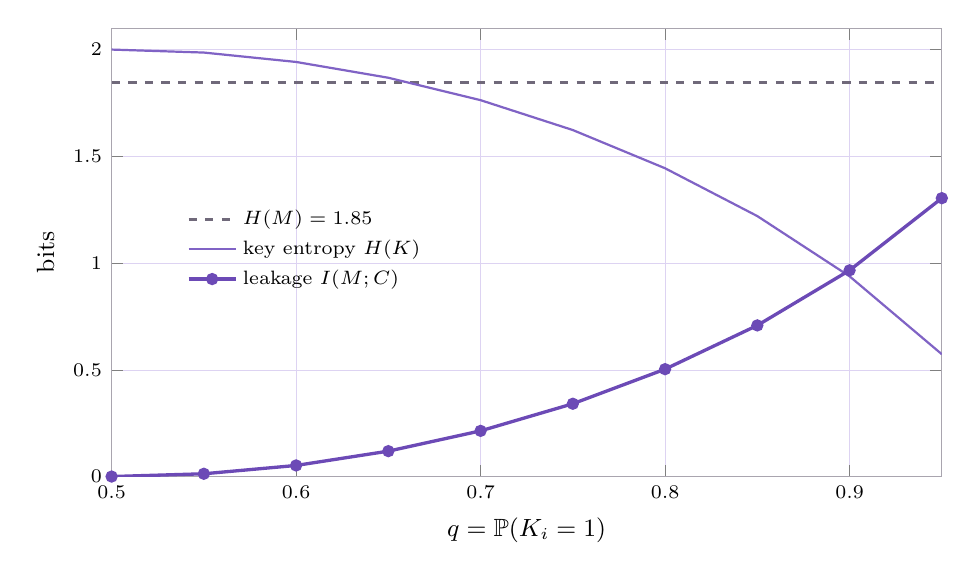
\begin{tikzpicture}
        \begin{axis}[
          width=\textwidth,height=0.6\textwidth,
          xlabel={$q=\Prob{K_i=1}$},ylabel={bits},
          xmin=0.5,xmax=0.95,ymin=0,ymax=2.1,
          xtick={0.5,0.6,...,0.9},
          legend style={at={(0.08,0.62)},anchor=north west},legend cell align=left,
          legend style={font=\scriptsize,draw=none,fill=none},
          tick label style={font=\scriptsize},
          label style={font=\small},
          axis line style={muted!60},
          grid=major,grid style={very thin,lavender}]
          \addplot[thick,dashed,muted] coordinates {(0.5,1.846) (0.95,1.846)};
          \addlegendentry{$\Ent{\msg}=1.85$}
          \addplot[thick,secondary] coordinates {
            (0.50,2.000) (0.55,1.986) (0.60,1.942) (0.65,1.868)
            (0.70,1.763) (0.75,1.623) (0.80,1.444) (0.85,1.220)
            (0.90,0.938) (0.95,0.573)};
          \addlegendentry{key entropy $\Ent{\key}$}
          \addplot[very thick,primary,mark=*,mark size=1.6pt] coordinates {
            (0.50,0.000) (0.55,0.013) (0.60,0.052) (0.65,0.119)
            (0.70,0.214) (0.75,0.341) (0.80,0.503) (0.85,0.708)
            (0.90,0.966) (0.95,1.304)};
          \addlegendentry{leakage $\MI{\msg}{\ctxt}$}
        \end{axis}
      \end{tikzpicture}
    \end{column}
    \begin{column}{0.42\textwidth}
      \textbf{\color{deep}$q=0.50$}\quad $\Ent{\key}=2$, $\MI{\msg}{\ctxt}=0$.

      \textbf{\color{deep}$q=0.95$}\quad $\Ent{\key}\approx0.57$,
      $\MI{\msg}{\ctxt}\approx1.30$ of the $1.85$ bits in $\msg$.
      \medskip

      For XOR with an independent key,
      $\MI{\msg}{\ctxt}=\Ent{\ctxt}-\Ent{\key}$.
      \medskip

      {\small A result for \emph{this} cipher, message distribution and
      key family. Key entropy alone does not decide security in general.\par}
    \end{column}
  \end{columns}
\end{frame}

% 14. Validation: simulation is planned, not done. Say so.
\begin{frame}{Checking the curve by simulation}
  \framesubtitle{Planned validation. The plot on the previous slide is theory, not measurement.}
  For each $q$:
  \begin{enumerate}
    \item sample messages from $(0.4,\,0.3,\,0.2,\,0.1)$
    \item sample independent $\Bern(q)$ key bits
    \item compute $\ctxt=\msg\xor\key$
    \item repeat about $10{,}000$ times and count the $(\msg,\ctxt)$ pairs
    \item estimate $\MI{\msg}{\ctxt}$ from the counts
    \item compare with the exact curve
  \end{enumerate}
  \medskip
  A plug-in estimate from a finite table has sampling error and a small
  upward bias, so at $q=0.5$ it should sit slightly above zero and shrink as
  the sample grows. No simulated points exist yet.
\end{frame}

\subsection{Conclusion}

% 15. Conclusion: the three levels, three sentences, one closing line.
\begin{frame}{Does random mean secure?}
  \begin{center}
    
\begin{tikzpicture}[>={Straight Barb},
        lvl/.style={draw=deep,fill=verylight,rounded corners=4pt,thick,
                    text width=3.3cm,align=center,minimum height=1.1cm,
                    font=\bfseries\color{deep}},
        sub/.style={font=\small\color{muted},align=center}]
      \node[lvl] (a) {LOOKS RANDOM};
      \node[lvl,right=1.3cm of a] (b) {IS HARD TO PREDICT};
      \node[lvl,right=1.3cm of b] (c) {PROTECTS INFORMATION};
      \node[sub,below=0.2cm of a] {statistical properties};
      \node[sub,below=0.2cm of b] {attacker knowledge};
      \node[sub,below=0.2cm of c] {secrecy};
      \draw[->,primary,very thick] (a) -- (b);
      \draw[->,primary,very thick] (b) -- (c);
    \end{tikzpicture}
  \end{center}
  \vspace{0.5ex}
  \begin{itemize}
    \item Balanced output does not mean independence.
    \item Passing a few statistical tests does not establish unpredictability.
    \item Once the randomness is a key, predictability turns into
          information leakage.
  \end{itemize}
  \vspace{0.5ex}
  \callout{\textbf{\color{deep}Good randomness is necessary for secrecy,\\
    but looking random is not enough to establish security.}}
\end{frame}

% ===========================================================================
% Backup slides: not part of the 20-minute timing.
% ===========================================================================
\appendix
\section{Backup}

% B1. What a p-value is and is not.
\begin{frame}{Backup: what a $p$-value actually says}
  For an observed statistic $t$ under the null model $H_0$
  (independent fair bits):
  \keyeq{p=\Prob{T\text{ at least as extreme as }t\mid H_0}}
  \begin{itemize}
    \item Small $p$: data of this kind would be rare if $H_0$ held.
          Evidence against $H_0$.
    \item Large $p$: this statistic did not detect a departure on this sample.
    \item It is not $\Prob{H_0\mid\text{data}}$, and it says nothing about
          what an attacker can compute from the output.
  \end{itemize}
  \medskip
  For the frequency test, $T=X\sim\Bin(n,\tfrac12)$; for the runs test,
  $T=R-1\sim\Bin(n-1,\tfrac12)$. Both are two-sided.
  Standard batteries such as NIST SP 800-22 collect many such statistics.
\end{frame}

% B2. Markov details behind the "memory" slide.
\begin{frame}{Backup: the two-state Markov source}
  \textbf{Markov property.} $\Prob{B_{i+1}=b\mid B_1,\ldots,B_i}
  =\Prob{B_{i+1}=b\mid B_i}$: the future depends on the past only
  through the present bit.
  \medskip
  \[P=\begin{pmatrix}1-s&s\\ s&1-s\end{pmatrix},
    \qquad P_{ab}=\Prob{B_{i+1}=b\mid B_i=a}.\]
  \begin{itemize}
    \item Start with $\Prob{B_1=1}=\tfrac12$. By symmetry of $P$, every
          $B_i$ is $\Bern(\tfrac12)$, so the frequency statistic still has
          mean $n/2$.
    \item Each neighbouring pair switches independently with probability
          $s$, so $R-1\sim\Bin(n-1,s)$ and $\Ex{R}=1+(n-1)s$.
    \item A natural estimate is $\hat s=(R-1)/(n-1)$.
  \end{itemize}
  \medskip
  \small Blitzstein and Hwang, \emph{Introduction to Probability}, Ch.~11,
  for the Markov property and transition matrix. Nothing more of the chapter
  is needed here.
\end{frame}

% B3. The full posterior at q = 0.95, C = 11.
\begin{frame}{Backup: the posterior at $q=0.95$, $\ctxt=11$}
  Key probabilities: $\Prob{\key=00}=0.0025$, $\Prob{01}=\Prob{10}=0.0475$,
  $\Prob{11}=0.9025$. The key that maps $m$ to $c=11$ is $m\xor11$.
  \begin{center}
    \begin{tabular}{@{}cccc@{}}
      \toprule
      $m$ & $\Prob{\msg=m}$ & $\Prob{\key=m\xor11}$ & product \\
      \midrule
      00 & 0.40 & 0.9025 & 0.3610 \\
      01 & 0.30 & 0.0475 & 0.01425 \\
      10 & 0.20 & 0.0475 & 0.0095 \\
      11 & 0.10 & 0.0025 & 0.00025 \\
      \midrule
      & & $\Prob{\ctxt=11}$ & 0.3850 \\
      \bottomrule
    \end{tabular}
  \end{center}
  \[\Prob{\msg=00\mid\ctxt=11}=\frac{0.3610}{0.3850}\approx0.938,
    \qquad\text{versus the prior }0.40.\]
  Bayes' rule with the law of total probability in the denominator.
\end{frame}

% B4. A small deterministic generator, to make "recover the state" concrete.
\begin{frame}{Backup: a small deterministic generator}
  A linear congruential generator:
  \keyeq{X_{n+1}=(aX_n+c)\bmod m,\qquad B_n=X_n\bmod 2}
  \begin{itemize}
    \item The whole future is fixed by the state $X_n$ and the constants
          $(a,c,m)$.
    \item With a small $m$ an attacker can try every state and match the
          observed bits; from then on nothing is unknown.
    \item Its output may still look balanced and switch a reasonable amount
          on a short sample. That is the gap between passing a test and
          being unpredictable.
  \end{itemize}
  \medskip
  Cryptographic generators are also deterministic after seeding. The
  difference is a design goal: recovering the state or predicting the next
  bit should be computationally infeasible.
\end{frame}

% References.
\begin{frame}{References}
  \begin{itemize}
    \item J. K. Blitzstein and J. Hwang, \emph{Introduction to Probability},
          2nd ed. Bernoulli and Binomial distributions, conditional
          probability, Bayes' rule, Markov property.
    \item C. E. Shannon, ``A Mathematical Theory of Communication,'' 1948.
          Entropy and mutual information.
    \item C. E. Shannon, ``Communication Theory of Secrecy Systems,'' 1949.
          Perfect secrecy.
    \item NIST SP 800-22 Rev.\,1a, 2010. Statistical test suite for random
          and pseudorandom number generators.
  \end{itemize}
\end{frame}

\end{document}
